% This document is available under the Creative Commons Attribution-ShareAlike
% License; additional terms may apply. See
%   * http://creativecommons.org/licenses/by-sa/3.0/
%   * http://creativecommons.org/licenses/by-sa/3.0/legalcode
%
% Copyright 2010 Jérôme Pouiller <jezz@sysmic.org>
%

\part{Démarrer}

{
\setbeamertemplate{background canvas}{}
\begin{frame}[plain]
  \partpage
  \begin{textblock}{11}(5,10)
    %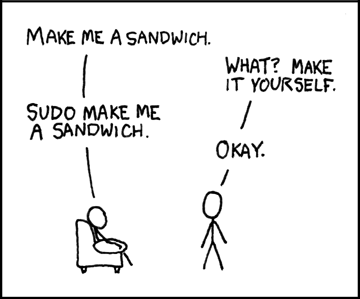
\includegraphics[height=30mm,width=30mm]{sandwich}
    \begin{quote}
      \rmfamily\textit\textbf\color{darkgray}{\large
        ``The first 90 percent of the code accounts for the first 90 percent of the
        development time. The remaining 10 percent of the code accounts for the
        other 90 percent of the development time''}
      \vskip3mm\hspace*\fill{\small--- Tom Cargill, Bell Labs}
    \end{quote}
  \end{textblock}
\end{frame}
}

\begin{frame}
  \tableofcontents
\end{frame}

\section{Le Boot}

\begin{frame}[fragile=singleslide]{Le Boot}
  Les Bootloaders:
  \begin{itemize}
  \item Le CPU commence par  executer des instructions situées sur une
    addresse mémoire.
  \item  Le  premier  morceau  de  code se  trouve  forcément  mappé
    directement en mémoire
  \item Il  s'agit généralement d'une eeprom ou  d'une rom (Celle-ci
    est directement  mappée sur  le bus d'adresse,  contrairement au
    flash)
  \item   De    nos   jours   les    micro-controlleur   intègre   des
    \emph{bootloader} en ROM
  \item   Ces   bootloader   peuvent   peuvent  avoir   de   nombreuse
    fonctionnalités
  \item Les ROM ont  généralement une capacité limitée (entre quelques
    Ko et quelques Mo)
  \end{itemize}
\end{frame}

\begin{frame}[fragile=singleslide]{Le Boot}
  \begin{itemize}
  \item L'objectif du premier étage est de charger la suite du système
    en mémoire
    \begin{itemize}
    \item Initialiser un périphérique plus important comme une flash
    \item Copier le contenu du périphérique en mémoire
    \item Sauter sur le bootloader de niveau suivant
    \end{itemize}
  \item Il existe souvent plusieurs étage de bootloader
  \item A la  fin de l'éxecution des bootloaders,  le noyau du système
    d'exploitation doit être présent en mémoire.
  \end{itemize}
\end{frame}

\begin{frame}[fragile=singleslide]{Le Boot}
  Le noyau:
  \begin{itemize}
  \item Généralement compressé.
  \item Le  noyau contient un  bootloader qui décompresse le  noyau en
    mémoire
  \item       Démarrage       de       Linux      proprement       dit
    (\file{init/main.c:start_kernel}).
  \item   Initilisation  des  parties   primordiales  de   l'OS:  MMU,
    scheduler,...
  \item Le noyau cherche à démarrer un programme pour donner la main à
    l'utilisateur.
  \item Il  faut tout d'abord initialiser le  périphérique de stockage
    (disque dur, flash, etc...).
  \item Il le monte sur \file{/} puis il démarre \file{/sbin/init}.
  \end{itemize}
\end{frame}

\begin{frame}[fragile=singleslide]{Le Boot}
  L'espace utilisateur:
  \begin{itemize}
  \item \file{/sbin/init}:  Execute \file{/etc/init.d/rcS}
  \item qui  éxecute \file{/etc/rc2.d/*}.  Ces  scripts contiennent le
    démarrage de divers applications.
  \item  ...  et  en  particulier \file{login}  ou  de \file{gdm}  qui
    permet  à  l'utilisateur  de  s'authentifier et  d'intéragir  avec
    Linux.
  \end{itemize}
\end{frame}

\begin{frame}[fragile=singleslide]{Exemples}
  Exemple de système Linux SysV sur Atmel SAM926 (Arm 926ejs):
    \begin{itemize}
    \item  ROMBoot:  Execution  de  ROMBoot,  depuis  la  ROM  sur  le
      microcontrolleur.   ROMBoot  intègre  un  système  verifiant  le
      premier octet de l'EEprom. Si  celui-ci vaut 0, il attend sur le
      port serie des octets qu'il ecrira sur l'eeprom
    \item AT91Bootstrap: ROMBoot passe  la main à AT91Bootstrap qui se
      trouve sur  une EEPROM. AT91Bootstrap peut  initialiser la flash
      et charger le contenu des premières pages
    \item U-Boot:  Ces pages contiennent U-Boot,  un bootloader évolué
      capable  d'initialiser  le  port  RS232,  le  réseau,  lire  des
      partitions, des fichiers, etc...
    \item  Bootloader   Noyau:  U-Boot   charge  le  noyau   linux  en
      mémoire.  Celui-ci est  compressé.  Un  bootloader permet  de le
      décompresser (head.S).
    \item    Noyau:     Démarrage    de    Linux
    \item   \file{/sbin/init}:   Execute  \file{/etc/init.d/rcS}   qui
      éxecute \file{/etc/rc2.d/*}.  ce script contiennent le démarrage
      de divers application et  en particulier \file{login} qui permet
      à l'utilisateur de s'authentifier et d'intéragit avec Linux.
    \end{itemize}
\end{frame}

\begin{frame}[fragile=singleslide]{Exemples}
  Exemple du système Linux sur imx6 (Arm Cortex-A9):
  \begin{itemize}
  \item Le bootloader situé en ROM lis une configuration enfonction de
    l'état  de  certains GPIO.   Cette  configuration  lui indique  de
    charger une  carte SD.  Il initialise  le bus, puis  le lecteur de
    carte et copie les première pages de la carte SD en mémoire.
  \item  Les  premières  pages  sont  assez  large  pour  contenir  le
    noyau. Le noyau est executé
  \item Le noyau démarre ensuite comme sur le SAM926
  \end{itemize}
\end{frame}

\begin{frame}[fragile=singleslide]{Exemples} Exemple sur PC-Bios
  \begin{itemize}
  \item Un bootloader  est executé depuis une ROM sur  le CPU. Il fait
    une initialisation très bas niveau du CPU.
  \item Le bootloader  donne la main au bios situé  sur une EEPROM. Le
    bios contient la configuration du périphérique à executer
  \item Le Bios charge les 512 premiers octets du disque configuré. Il
    s'agit du premier étage de Grub
  \item  En s'appuyant  sur  les  fonctions données  par  le Bios,  le
    premier étage de Grub charge l'étage 1.5 contenant 30Ko de données
    un peu après le MBR.
  \item L'étage 1.5 va  chercher le fichier \file{/boot/grub} (l'étage
    2)  et le charge.   L'étage 2  est capable  d'afficher un  menu et
    d'intéragir avec l'utilisateur.
  \item L'étage charge \file{/boot/vmlinuz}.
  \item Le bootloader du noyau se décompresse le noyau en mémoire.
  \item La suite est identique aux autres boot.
  \end{itemize}
 \end{frame}

\subsection{Booter par réseau}

\begin{frame}{Booter par réseau}
  \begin{itemize}
  \item Permet de travailler  plus confortablement car evite les cycles
    de scp/flash
  \item Parfois, il faut demarrer  la cible sous Linux pour pouvoir la
    flasher.  C'est donc la seule manière de continuer.
  \item Fonctionne aussi très bien avec des PC
  \item Trois étapes pour démarrer un système
    \begin{enumerate}
    \item Le bootloader configure la carte réseau et place le noyau en
      mémoire
    \item Le noyau s'execute et monte un filesystem réseau
    \item Le premier processus de la vie du système est lancé: \cmd{init}
    \end{enumerate}
    \end{itemize}
\end{frame}

\section{Le bootloader}

\begin{frame}[fragile=singleslide]{Le bootloader}{Description}
  \begin{itemize}
  \item    Le    bootloader     se    trouver    souvent    sur    une
    \emph{eeprom}.  Celle-ci   est  directement  mappée   sur  le  bus
    d'adresse
  \item Au minimum, il doit initialiser:
    \begin{itemize}
    \item les timing de la mémoire RAM
    \item les caches CPU
    \end{itemize}
  \end{itemize}
\end{frame}

\begin{frame}[fragile=singleslide]{Le bootloader}{Description}
  \begin{itemize}
  \item Il peut :
    \begin{itemize}
    \item Initialiser une ligne série pour l'utiliser comme terminal
    \item Offrir un prompt et accèder à des options de boot
    \item Initialiser la mémoire flash
    \item Copier le noyau en mémoire
    \item Passer des arguments au noyau
    \item Initialiser le chipset réseau
    \item  Récupérer  des  informations  provenant d'un  serveur  DHCP
      (serveur où récupérer l'image du noyau, indications sur les mise
      à jour disponibles, etc...)
    \item Lire des fichiers provenant du réseau
    \item Lire des fichier par \verb+{X,Y,Z}MODEM+
    \item Ecrire sur la flash
    \item Gérer un système de secours
    \item  Initialiser des  fonctionnalités  cryptographiques (Trusted
      Plateform Manager)
    \end{itemize}
  \end{itemize}
\end{frame}

\begin{frame}{Le bootloader}{Description}
  \begin{itemize}
    \item Il  est très  rare de pouvoir  démarrer Linux  sans bootloader
    fonctionnel
    \item Si votre bootloader  n'est pas fonctionnel, vous aurez souvent
    besoin d'un matériel particulier pour  le mettre à jour (un outils
    capable de flasher l'eeprom)
  \end{itemize}
  Bootloader connus:
  \begin{itemize}
    \item Grub
    \item Syslinux (et son dérivé Isolinux)
    \item U-Boot
    \item Redboot
    \item BareBox (successeur de U-Boot)
  \end{itemize}
\end{frame}

\begin{frame}[fragile=singleslide]{Le bootloader}{Test}
  Testons notre bootloader:
  \begin{itemize}
    \item Démarrez minicom
    \begin{lstlisting}
host$ minicom -D /dev/ttyUSB1
    \end{lstlisting}
  \item Resettez la carte
  \item Appuyez sur une touche pour stopper le démarrage
    \begin{lstlisting}
[...]
Hit any key to stop autoboot:  0
    \end{lstlisting}
  \item Obtenez la liste des commandes
    \begin{lstlisting}
uboot> help
    \end{lstlisting}
  \end{itemize}
  Attention:
  \begin{itemize}
  \item Pas d'historique
  \item Pas de flèches gauche/droite
  \end{itemize}
  En  cas de  problème pour  vous connecter,  vérifiez  vos paramètres
  RS232.
\end{frame}

\subsection{TFTP}

\begin{frame}[fragile=singleslide]{TFTP}{Mise en place}
  \begin{itemize}
  \item Identique au protocole \cmd{ftp} mais plus simple
  \item Permet d'etre implémenté avec très peu de ressource
  \item Mise en place:
    \begin{lstlisting}
host% apt-get install tftp-hpa tftpd-hpa
host% cp hello/build-arm/hello /srv/tftp
    \end{lstlisting}
  \item Test en local
    \begin{itemize}
    \item Par le shell interactif
      \begin{lstlisting}
host$ tftp 127.0.0.1
> get hello
> quit
      \end{lstlisting}
    \item Par la ligne de commande
      \begin{lstlisting}
host$ tftp 127.0.0.1 -c get hello
      \end{lstlisting} % $
    \end{itemize}
    \note[item]{Il est possible de parler de inetd et /etc/default/atftpd}
  \item En cas de  problème, consultez les logs (\file{/var/log/syslog}
    ou \file{/var/log/daemon.log})
% A priori, ca n'est plus vrai avec les nouvelles version:
%     \item Remarque: chemin absolu, pas de cd, etc...
%       \begin{lstlisting}
% host$ scp root@target:/.../uImage /var/lib/tftpboot
% host$ atftp 127.0.0.1 -g -l /var/lib/tftpboot/uImage # Test
%       \end{lstlisting}
  % \item En  cas d'utilisation intensive (déploiement  sur des milliers
  %   de  systèmes),  vous   pouvez  utiliser  \cmd{atftpd}  de  manière
  %   autonome (voir \file{/etc/default/atftpd})
  % \item  Il  est  possible  de  modifier le  répertoire  partagé  dans
  %   \file{/etc/inetd.conf} ou dans \file{/etc/default/atftpd} (suivant
  %   le mode d'éxecution)
  %   \note[item]{Parler de inetd}
  \item  Il  est  possible  de  modifier le  répertoire  partagé  dans
    \file{/etc/default/tftpd-hpa}
  \end{itemize}
\end{frame}

\begin{frame}[fragile=singleslide]{TFTP}
  \note[item]{Il faut fournir le noyau pré-compilé ou le noyau Calao}
  Configuration de la cible pour télécharger et démarrer le noyau. Par RS232:
  \begin{itemize}
  \item Configuration de l'IP
    \begin{lstlisting}
uboot> setenv ipaddr 192.168.1.12
    \end{lstlisting}
  \item Vérification la configuration IP
    \note[item]{U-boot n'est  pas assez évolué pour  répondre aux ping
      (ca nécessite un service qui tourne en arrière plan ce qui n'est
      pas souhaitable pour faire du debug de bas niveau)}
    \begin{lstlisting}
uboot> ping 192.168.1.10
    \end{lstlisting}
  \item Déclaration de notre \emph{host} comme serveur \cmd{tftp}
    \begin{lstlisting}
uboot> setenv serverip 192.168.1.10
uboot> saveenv
    \end{lstlisting}
    \note[item]{Eventuellement,   rebooter  après   le   saveenv  pour
      initialiser correctement le réseau}
  \item Téléchargement du noyau dans une zone libre de la mémoire
    \note[item]{Expliquer d'où provient 21000000}
    \note[item]{L'adresse de  chargement du noyau  dépend de plusieurs
      parmètres: topologie  mémoire, utilisation  de la m'oire  par le
      bootloader, configuration du noyau, taille du noyau, etc..}
%    \note[item]{Reprendre   un    schéma   similaire   à    celui   de
%      \verb+http://www.at91.com/linux4sam/bin/view/Linux4SAM/GettingStarted#Linux4SAM_NandFlash_demo_Memory+
%      mais pour la RAM}
    \begin{lstlisting}
uboot> tftpboot 21000000 uImage
    \end{lstlisting}
  \item Exécution du noyau
    \begin{lstlisting}
uboot> bootm 21000000
    \end{lstlisting}
    \note[item]{Si autostart=yes, pas besoin de cette derniere ligne}
  \item Le noyau  trouve la flash, monte la flash  et charge l'init de
    la flash
    \note[item]{Exo: faites la même chose par ZMODEM}
    \note[item]{Tester avec le NFS éteind}
  \end{itemize}
\end{frame}

\subsection{NFS}

\begin{frame}[fragile=singleslide]{Nfs}
  Comparable au partage réseau de windows.
  \begin{itemize}
  \item Installation
    \begin{lstlisting}
host% apt-get install nfs-kernel-server nfs-common
host$ mkdir nfs-root
host% vim /etc/exports
    \end{lstlisting} % $
    \note[item]{nfs-common contient le client}
    \note[item]{On peut essayer avec unfs3}
    \note[item]{Autrefois le paquet s'apellait nfs-user-serveur}
  \item Configuration du partage
    \begin{lstlisting}
/home/user/nfs-root 0.0.0.0/0.0.0.0(ro,no_root_squash)
    \end{lstlisting}
  \end{itemize}
\end{frame}

\begin{frame}[fragile=singleslide]{Nfs}
  \begin{itemize}
    \item Test sur l'hôte
      \begin{lstlisting}
host% service nfs-kernel-server restart
host$ mkdir nfs-mount
host% mount -t nfs 127.0.0.1:/home/user/nfs-root nfs-mount
      \end{lstlisting} % $
    \item Vérification des droits root
      \begin{lstlisting}
host$ echo foo > nfs-root/file
host$ chmod 000 nfs-root/file
host$ ls -l nfs-mount
host% cat nfs-mount/file
      \end{lstlisting} % $
      \note[item]{ Le  test sur la cible  ne fonctionne que  si les binaires
        necessaires sont installée}
     \item Test sur la cible (nécessite le support de NFS dans \cmd{mount})
       \begin{lstlisting}
target$ mkdir nfs-mount
target% mount -t nfs 192.168.1.10:/home/user/nfs-root nfs-mount
       \end{lstlisting} % $
     \item En cas de problème, vérifiez les logs: \file{/var/log/daemon.log}
   \end{itemize}
\end{frame}

%    \note[item] {Ca permet de ne pas leur donner le rootfs. Est-ce qu'on garde?}
%    \note[item] {C'est une très mauvaise idée de dumper une partition montée}
%    \note[item] {Il faut mieux leur faire faire cette manip dans la section sur les MTD}
%     \item Obtenir une copie conforme de la cible
%       \begin{lstlisting}
% target% tar cv / | tftp host -p -l - -r /srv/tftp/root.tar
% host$ gzip /srv/tftp/root.tar
%       \end{lstlisting} % $
\begin{frame}[fragile=singleslide]{Démarrage sur le NFS}
  \begin{itemize}
  \item Modification des arguments passés au noyau
    \note[item]{Testé avec 3e83c0851c2f1483ef92ce845e6f27e3 uImage, du
      site de Calao}
    \note[item]{Testé       avec      50ddb3a654f5e56e3fa1a70216abbb5e
      rootfs.arm.jffs2 du site de Calao}
    \begin{itemize}
    \item Configuration IP
      \begin{lstlisting}
uboot> setenv ipconf ip=192.168.1.13:192.168.1.10:192.168.1.254:255.255.255.0:target:eth0:off
      \end{lstlisting}
    \item Configuration NFS
      \begin{lstlisting}
uboot> setenv nfsconf root=/dev/nfs nfsroot=/home/user/nfs-root
      \end{lstlisting}
    \item La variable \cmd{bootargs} permet de passer des arguments au noyau
      \begin{lstlisting}
uboot> setenv bootargs ${ipconf} ${nfsconf} panic=1
      \end{lstlisting}
    \item Démarrage
      \begin{lstlisting}
uboot> boot
      \end{lstlisting}
    \end{itemize}
  \item Voir \file{Documentation/filesystem/nfs/nfsroot.txt}
  \item Après avoir monté le NFS, le noyau essaye de passer la main au
    programme \cmd{init}
  \end{itemize}
\end{frame}

\section{Flasher le rootfs}

\begin{frame}[fragile=singleslide]{Création du rootfs}
  Pour créer une image \cmd{jffs2}, vous devez au minimum spécifier le
  répertoire  de source,  l'image de  destination, l'endianness  et le
  padding:
  \begin{lstlisting}
target% cat /proc/mtd
host% apt-get install mtd-utils
host$ mkfs.jffs2 -l -p -r nfs-root -o rootfs.jffs2
  \end{lstlisting}
  Afin de rendre notre image  plus performante, ajustons la taille des
  pages,  supprimons  les  cleanmarkers  (on pourrait  aussi  utiliser
  \verb+-c 0+) et changeons le propriétaires des fichier en root:
  \begin{lstlisting}
host$ mkfs.jffs2 -l -p -q -n -s 2048 -e 128 -r nfs-root -o rootfs.jffs2
  \end{lstlisting}
\end{frame}

\begin{frame}[fragile=singleslide]{Recopier le système sur la flash}
  Le  plus  générique pour  recopier  la flash  sur  la  cible est  de
  démarrer Linux par un autre moyen  (NFS ou partition de rescue) et d
  utiliser les outils Linux.
  \begin{itemize}
  \item Toujours commencer par effacer le contenu précédent (on risque
    sinon des corruptions sur le filesystem)
    \begin{lstlisting}
target% flash_eraseall /dev/mtd1
target% cd /tmp
    \end{lstlisting}
  \item    Il   existe   des    fichiers   devices    \verb+mtd*+   et
    \verb+mtdblock*+:
    \begin{itemize}
    \item Les fichiers block ne sont la que pour la compatibilité avec
      certains outils.  Ils ne gèrent  pas les \emph{badblock}  et les
      \emph{clean markers}.
    \item  Il  est préférable  de  passer  le  plus possible  par  les
      fichiers \verb+mtd*+
    \item  Les  flashs  doivent   être  écrite  en  prenant  certaines
      precautions (padding  sur les pages, etc...).  Il est préférable
      de systématiquement écrire en utilisant les outils spécialisés
    \end{itemize}
  \end{itemize}
\end{frame}

\begin{frame}[fragile=singleslide]{Recopier le système sur la flash}
  \begin{itemize}
  \item Téléchargeons  le rootfs sur  notre cible. Nous  pouvons avoir
    des problèmes  de place pour stoker  cette image.  Il  est dans ce
    cas préférable de  travailler sur NFS (mais ca  n'est pas toujours
    possible).
    \begin{lstlisting}
target% tftp -g -r rootfs.jffs2
target% nandwrite -p /dev/mtd1 rootfs.jffs2
    \end{lstlisting}
    ou bien
    \begin{lstlisting}
host$ serve_image 0.0.0.0 1234 rootfs.jffs2 128
target% recv_image host 1234 /dev/mtd1
    \end{lstlisting}
  \item  Test
    \begin{lstlisting}
target% mkdir /tmp/mtd1
target% mount -t jffs2 /dev/mtdblock1 /tmp/mtd1
    \end{lstlisting}
  \end{itemize}
\end{frame}

\begin{frame}[fragile=singleslide]{Recopier le système sur la flash}
  Il est possible d'effectuer cette opération à partir de U-Boot.
  \begin{itemize}
  \item Nous allons utiliser TFTP sans démarrer dessous. Désactivons l'autostart
    \begin{lstlisting}
uboot> set autostart no
    \end{lstlisting}
  \item Toujours effacer toute la partition avant de flasher
    \begin{lstlisting}
uboot> nand erase clean 1000000 8800000
    \end{lstlisting}
  \item On place l'image en mémoire afin de la flasher
    \begin{lstlisting}
uboot> tftp 21000000 rootfs.arm.jffs2
uboot> nand write 21000000 1000000 $filesize
    \end{lstlisting}
  \end{itemize}
\end{frame}

\begin{frame}[fragile=singleslide]{Recopier le noyau sur la flash}
  L'opération est similaire au filesystem. Dans la plupart des cas, on
  place le  noyau à  part sur  une autre partition  de la  flash. Nous
  n'avons alors pas besoin de filesystem:
  \begin{itemize}
  \item Sous Linux
    \begin{lstlisting}
target% flash_erase /dev/mtd0 0x400000 0
target% cd /tmp
target% tftp -g -r uImage
target% nandwrite -s 0x400000 -p /dev/mtd0 uImage
    \end{lstlisting}
  \item Sous U-boot
    \begin{lstlisting}
uboot> tftp 21000000 uImage
uboot> nand erase clean 400000 200000
uboot> nand write 21000000 400000 $filesize
    \end{lstlisting}
  \end{itemize}
\end{frame}

% \begin{frame}[fragile=singleslide]{Automatisation}
%   Les  options  non utilisées  par  le  noyau  sont passée  au  script
%   d'initialisation.   Ajoutons  une   option  permettant   de  flasher
%   automatiquement notre cible:
%   \begin{lstlisting}
% if [ $1 == FLASH ]
%   flash_eraseall /dev/mtd0
%   flash_eraseall /dev/mtd1
%   cd /tmp
%   nandwrite -p /dev/mtd0 uImage
%   nandwrite -p /dev/mtd1 rootfs.jffs2
% fi
%   \end{lstlisting}
% \end{frame}

% Ajouter partie sur UBIFS
\begin{frame}[fragile=singleslide]{Ubifs}
  \begin{itemize}
  \item Ubi ajoute une couche d'abstraction à la flash
  \item Il a le même rôle que controlleur matériel de mémoire flash sur les clefs USB
  \item Ubi est géré en volume. A l'intérieur d'un volume, il est possible d'avoir plusieurs partition
  \item Ubifs est un filesystem qui optimise les accès à la flash au dessus d'UBI
  \end{itemize}
\end{frame}

\begin{frame}[fragile=singleslide]{Ubifs}
  \begin{itemize}
  \item Création d'une partition Ubifs:
    \begin{lstlisting}
host% mkfs.ubifs -m 2048 -e 128KiB -c 960 -d /home/user/nfs -o rootfs.ubifs
     \end{lstlisting}
  \item Integration dans un volume UBI:
    \begin{lstlisting}
host$ cat <<EOF > ubinize.cfg
>[rootfs]
>mode=ubi
>image=rootfs.ubifs
>vol_id=0
>vol_type=dynamic
>vol_name=rootfs
>vol_alignment=1
EOF
host$ ubinize -p 128KiB -m 2048 -o rootfs.ubi /tmp/ubinize.cfg
     \end{lstlisting}
  \end{itemize}
\end{frame}

\begin{frame}[fragile=singleslide]{Ubifs}
  \begin{itemize}
  \item Flashage.
    \begin{lstlisting}
target% nandwrite -p /dev/mtd1 rootfs.ubi
     \end{lstlisting}
  \item Flashage alternatif. Remarquez que l'utilisation de ubiformat permet de
    conserver les \emph{erase counters}
    \begin{lstlisting}
target% ubiformat /dev/mtd1 -f rootfs.ubi
     \end{lstlisting}
  \item On peut maintenant monter le volume puis la partition
    \begin{lstlisting}
target% ubiattach /dev/ubi_ctrl -m 1
target% mount -t ubifs /dev/ubi0_0 /tmp/ubi0
     \end{lstlisting}
     \item Remarquez que le volume doit être attaché avant de pouvoir monter la
       partition. Du coup, démarrer sur une partition ubifs possède une syntaxe
       particulière:
    \begin{lstlisting}
ubi.mtd=rootfs rootfstype=ubifs root=ubi0:0
     \end{lstlisting}
  \end{itemize}
\end{frame}

\begin{frame}[fragile=singleslide]{Monter le rootfs sur l'hôte}
  L'hôte  ne possèdant  pas  de  flash, nous  devons  la simuler  pour
  pouvoir monter le rootfs:
  \begin{itemize}
  \item  Chargeons le  module  permettant l'émulation  d'une flash  et
    copions notre image sur la flash virtuelle
    \begin{lstlisting}
host% modprobe nandsim cache_file=/home/user/flash first_id_byte=0x20 second_id_byte=0xaa third_id_byte=0x00 fourth_id_byte=0x15 parts=128,960,960
host% nandwrite -p /dev/mtd1 rootfs.jffs2
# ou: nandwrite -p /dev/mtd1 rootfs.ubifs
     \end{lstlisting}
  \end{itemize}
\end{frame}

\begin{frame}[fragile=singleslide]{Monter le rootfs sur l'hôte}
  \begin{itemize}
\item La suite est classique
    \begin{lstlisting}
host% modprobe mtdblock
host% mkdir /tmp/mtd1
host% mount -t jffs2 /dev/mtdblock1 /tmp/mtd1
     \end{lstlisting}
     \item ... ou...
    \begin{lstlisting}
host% mkdir /tmp/ubi1
host% ubiattach /dev/ubi_ctrl -m 1
host% mount -t ubifs /dev/ubi0_0 /tmp/ubi1
     \end{lstlisting}
  \end{itemize}
\end{frame}

% Obsolete:
% \begin{frame}[fragile=singleslide]{Monter le rootfs sur l'hôte}
%   L'hôte  ne possèdant  pas  de  flash, nous  devons  la simuler  pour
%   pouvoir monter le rootfs:
%   \begin{itemize}
%   \item  Chargeons le  module  permettant l'émulation  d'une flash  et
%     copions notre image sur la flash virtuelle
%     \begin{lstlisting}
% host% modprobe mtdram total_size=65536 erase_size=256
% host% nandwrite -p /dev/mtd0 rootfs.jffs2
%     \end{lstlisting}
%   \item  Alternativement, il  est  possible de  directement mapper  un
%     fichier sur une flash avec \file{block2mtd}
%     \begin{lstlisting}
% host% losetup /dev/loop0 rootfs.jffs2
% host% modprobe block2mtd block2mtd=/dev/loop0
%     \end{lstlisting}
%   \end{itemize}
% \end{frame}
%
% \begin{frame}[fragile=singleslide]{Monter le rootfs sur l'hôte}
%   \begin{itemize}
%   \item Chargeons la couche d''emulation par block et le filesystem
%     \begin{lstlisting}
% host% modprobe mtdblock
% host% modprobe jffs2
%     \end{lstlisting}
%   \item Copie de notre image
%     \begin{lstlisting}
% host% mkdir jffs2-mount
% host% mount -t jffs2 /dev/mtdblock0 jffs2-mount
%     \end{lstlisting}
%   \end{itemize}
%   % http://wiki.maemo.org/Modifying_the_root_image
% \end{frame}

\note{Est-ce que l'on ne devrait pas placer les chapitre sur u-boot et SAm-BA ici? Je pense que oui}

\section{Initramfs}

\begin{frame}[fragile=singleslide]{Initramfs}
  \begin{itemize}
  \item Qu'est-ce qu'un initramfs?
  \item Un petit filesystème chargé en mémoire par le bootloader
  \item Successeur de initrd (plus complexe d'utilisation)
  \item Permet déffectuer des actions avant le lancement d'init
  \item Il devrait rester petit et ne s'utiliser que pour continuer le
    boot
  \item  Si  vous  intégrez  busybox  dans  votre  initramfs,  il  est
    préconisé  de  le compiler  en  statique  en  ne gardant  que  les
    composant utiles
  \item  Cas classique:  charger les  modules permettent  d'acceder au
    filesystème:
    \begin{itemize}
    \item M-Sys Disc-On-Chip
    \item Configuration RAID
    \item Configuration réseau pour booter en NFS
    \end{itemize}
  \item Dans notre cas, il n'est pas utile car nous n'avons pas besoin
    de charger de driver particuliers avant le démarrage
  \end{itemize}
\end{frame}

\begin{frame}[fragile=singleslide]{Initramfs}
  \begin{itemize}
  \item Création d'un rootfs vraiment minimal:
    \begin{lstlisting}
host$ mkdir initramfs
host$ cd initramfs
host% tar xf rootfs.tar
host% ln -s bin/busybox init
# ou: cp .../hello-arm-static init
host$ find . |  cpio -H newc -o | gzip > ../initramfs.gz
    \end{lstlisting}
  \item Comme l'image noyau, l'image initramfs doit être au format u-boot.
    \begin{lstlisting}
host$ mkimage -A arm -T ramdisk -d initramfs.gz initramfs.gz.img
host$ cp initramfs.gz.img /home/user/tftp
    \end{lstlisting}
  \end{itemize}
\end{frame}

\begin{frame}[fragile=singleslide]{Initramfs}
  \begin{itemize}
  \item  On  indique  l'adresse   du  ramfs  en  second  paramètre  de
    \cmd{bootm}. Evidement, le noyau doit être configuré pour utiliser
    le ramfs.
    \begin{lstlisting}
uboot> tftp 21000000 uImage
uboot> tftp 21300000 initramfs.gz.img
uboot> bootm 21000000 21300000
    \end{lstlisting}
  \end{itemize}
  \note[item]{TODO P1 A verifier, tester, completer}
\end{frame}
